% 5implementacja
\newpage

\section{Implementacja}

\paragraph{}
Przedstawioną metodę zaimplementowano w języku C++, przy użyciu elementów języka dodanych przy standaryzacji w wersji C++11/14. Wykorzystano również następujące biblioteki:
\begin{itemize}
	\item glm - (OpenGL Mathematics) biblioteka zawierająca funkcje i klasy wykorzystywane przy operacjach matematycznych. W zamyśle naśladuje zapis OpenGL Shading Language (GLSL).
	\item OpenGL - (ang. Open Graphics Library) API służące do tworzenia grafiki.
	\item GLEW - (OpenGL Extension Wrangler) biblioteka pomocna przy ładowaniu odpowiednich elementów biblioteki OpenGL.
	\item GLFW - biblioteka zawiera zestaw funkcji ułatwiających m.in. tworzenie okna dla aplikacji wykorzystujących OpenGL i obsługę urządzeń wejściowych (klawiatury, myszki, joysticka).
\end{itemize}
Kod źródłowy aplikacji dostępny jest w publicznym repozytorium kodu pod adresem:\\ \href{https://github.com/filu005/SPH}{https://github.com/filu005/SPH}.
\par


\begin{figure}
\subsection{Algorytm}
\subsubsection{Schemat blokowy aplikacji}

\centering
\caption{Diagram przebiegu symulacji płynu}
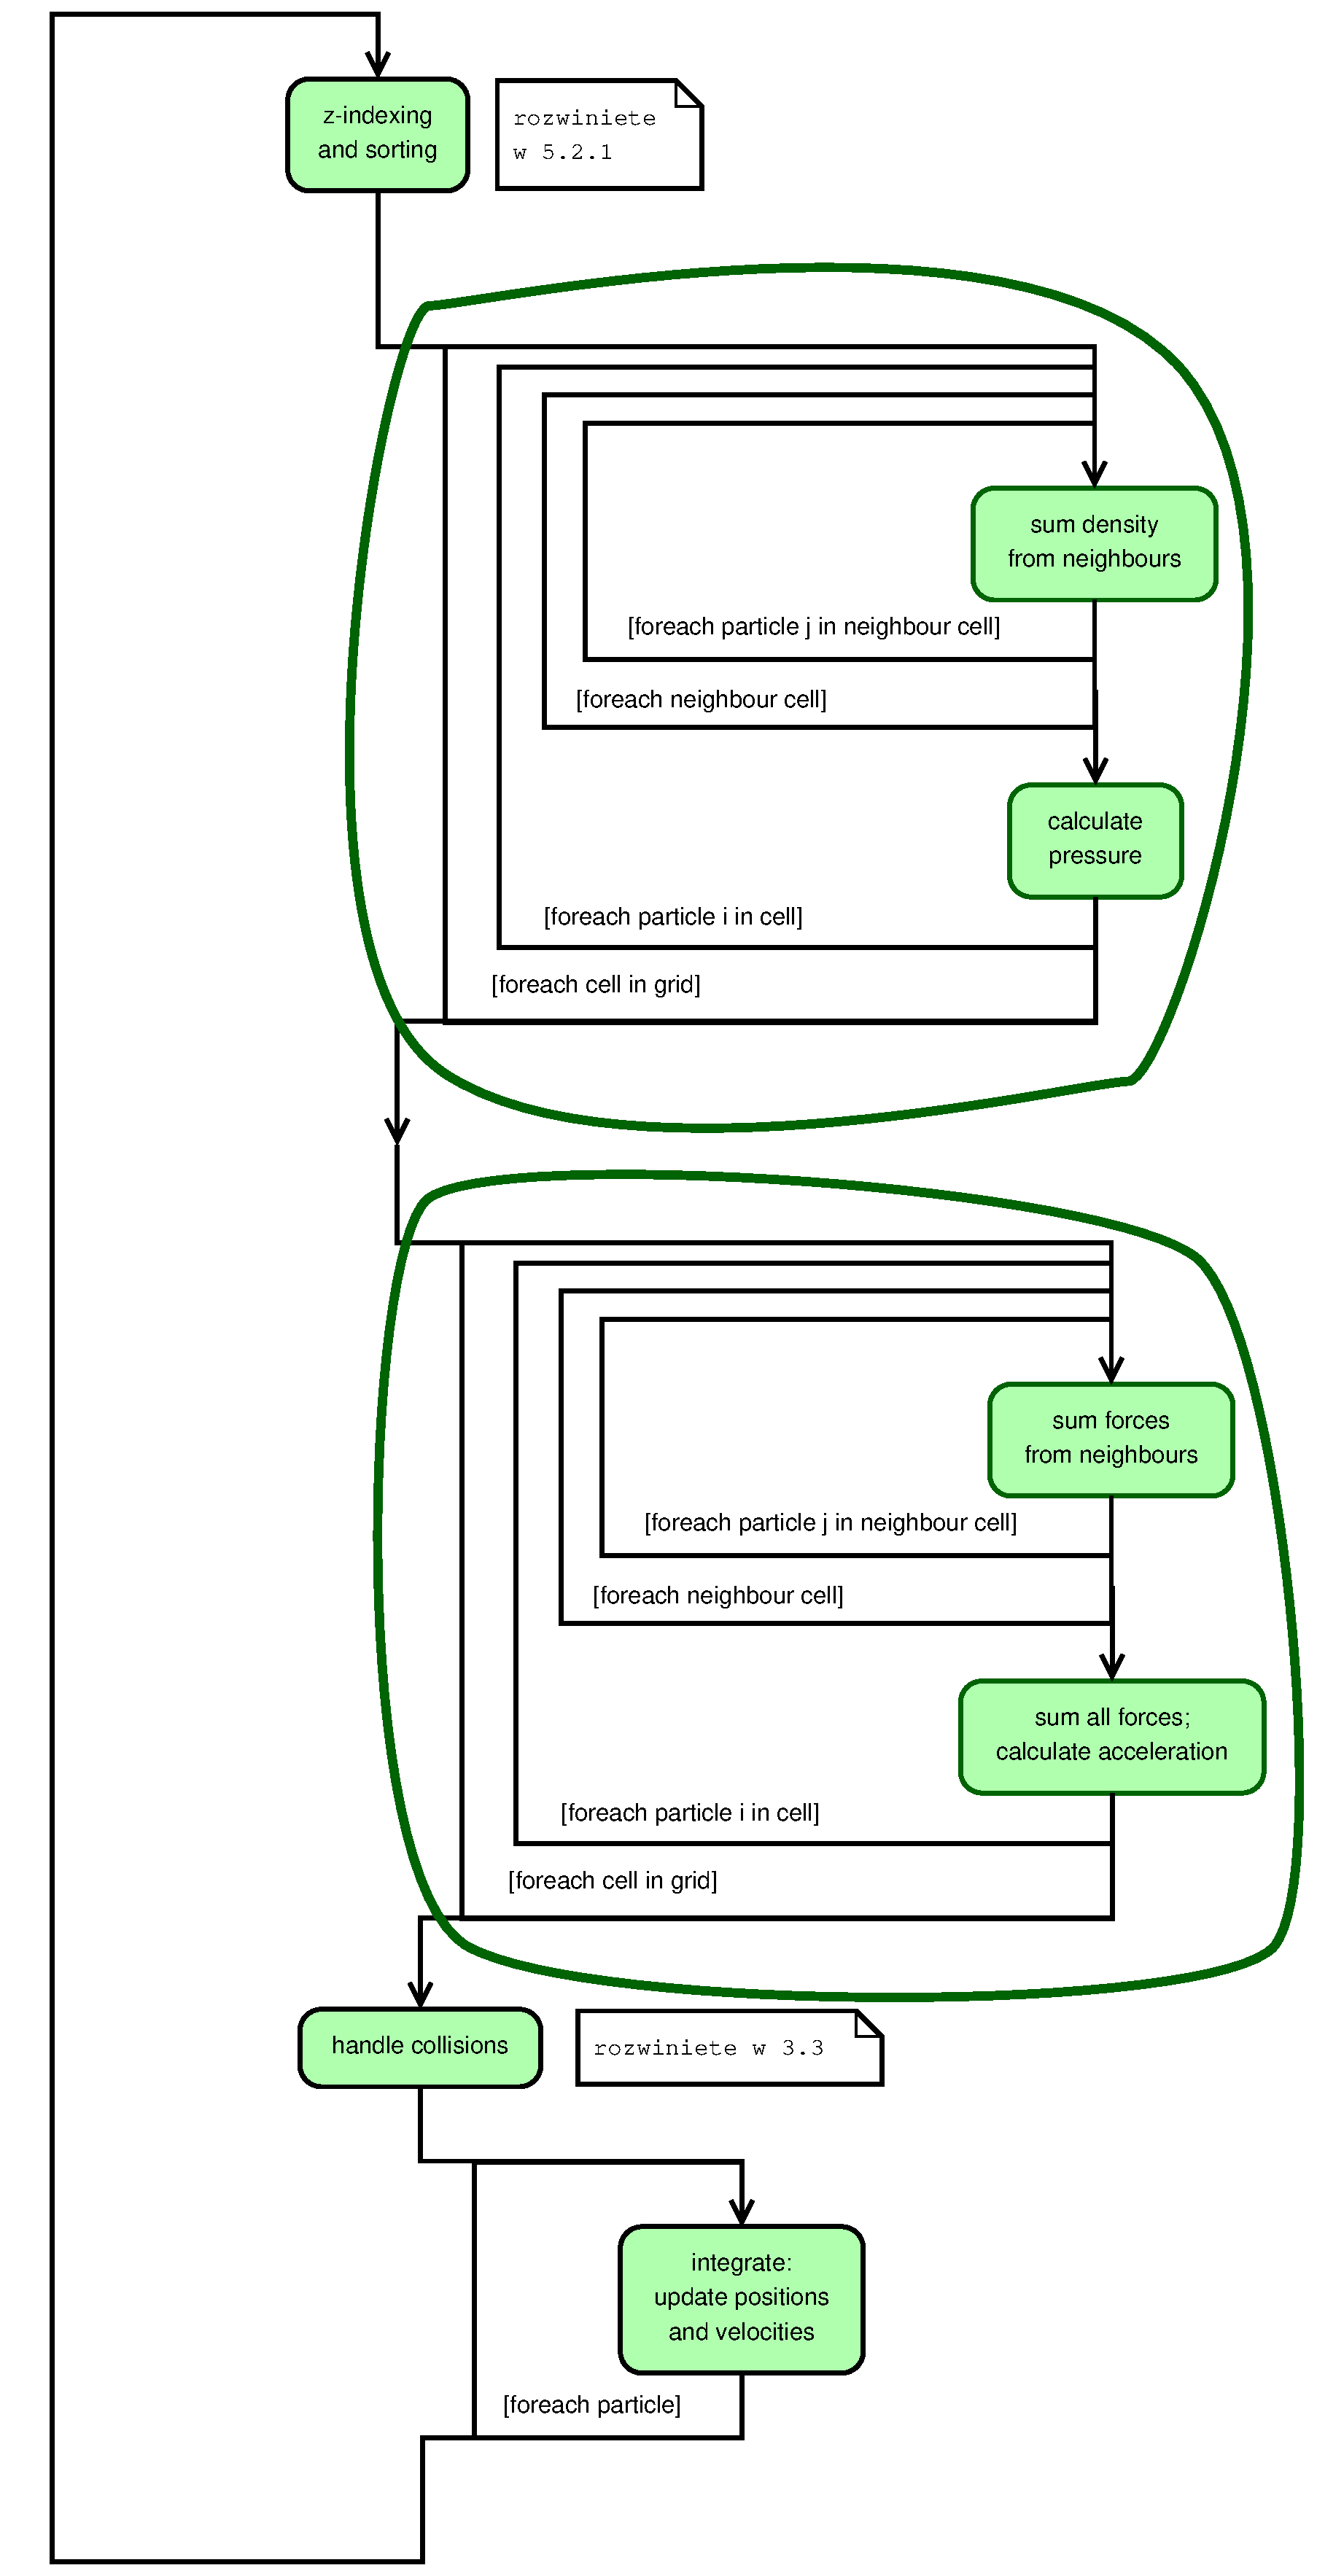
\includegraphics[width=350pt,keepaspectratio]{diagram.eps}%width=\textwidth,height=\textheight,
\label{fig:diagram_main}
\newpage
\end{figure}
\newpage

\subsubsection{Pseudokod algorytmu symulacji}

\paragraph{}
%\begin{figure}[H]
{
\setlength{\interspacetitleruled}{0pt}%
\setlength{\algotitleheightrule}{0pt}%
%\DecMargin{0.5em}
\begin{algorithm}[H]
%\SetAlgorithmName{Algorytm}{} %last arg is the title of listing table
	stwórz cząsteczki\;
	wyczyść siatkę sąsiadów\;
	posortuj cząsteczki według z-indeksów\;
	umieść cząsteczki na siatce\;
	\ForAll(\Comment*[f]{obliczenie gęstości}){komórek w siatce}
	{
		\ForEach{cząsteczki $i$ w komórce}
		{
			\ForEach{sąsiadującej komórki}
			{
				\ForEach{cząsteczki $j$ w sąsiadującej komórce}
				{
					$\rho_i(\boldsymbol{r}_i) \leftarrow \rho_i(\boldsymbol{r}_i) + m_j W(\boldsymbol{r}_i-\boldsymbol{r}_j, h)$
				}
			}
			$p_i \leftarrow k(({\rho_i \over \rho_0})^{7} - 1)$
		}
	
	}
	
	\ForAll(\Comment*[f]{obliczenie sił}){komórek w siatce}
	{
		\ForEach{cząsteczki $i$ w komórce}
		{
			\ForEach{sąsiadującej komórki}
			{
				\ForEach{cząsteczki $j$ w sąsiadującej komórce}
				{
					$\boldsymbol{F}_i^{cisn} \xleftarrow{i \neq j} \boldsymbol{F}_i^{cisn} - \rho_j m_j \left( {p_i \over \rho_i^2} + {p_j \over \rho_j^2} \right) \nabla W(\boldsymbol{r}_i-\boldsymbol{r}_j, h)$\\
					$\boldsymbol{F}_i^{lep} \leftarrow \boldsymbol{F}_i^{lep} + \mu {m_j \over \rho_j} (\boldsymbol{v}_i - \boldsymbol{v}_j) \nabla^2 W(\boldsymbol{r}_i-\boldsymbol{r}_j, h)$\\
					$\nabla{c}_S(\boldsymbol{r}_i) \leftarrow \nabla{c}_S(\boldsymbol{r}_i) + {m_j \over \rho_j} \nabla W(\boldsymbol{r}_i-\boldsymbol{r}_j, h)$\\
					$\nabla^2{c}_S(\boldsymbol{r}_i) \leftarrow \nabla^2{c}_S(\boldsymbol{r}_i) + {m_j \over \rho_j} \nabla^2 W(\boldsymbol{r}_i-\boldsymbol{r}_j, h)$
				}
			}
			\If{$\|\nabla{c}_S(\boldsymbol{r}_i)\| \geq l$}
			{
				$\boldsymbol{F}_i^{pow} \leftarrow -\sigma \nabla^2{c}_S(\boldsymbol{r}_i) {\nabla{c}_S(\boldsymbol{r}_i) \over \|\nabla{c}_S(\boldsymbol{r}_i)\|}$
			}
			$\boldsymbol{F}_i^{total} \leftarrow \boldsymbol{F}_i^{cisn} + \boldsymbol{F}_i^{lep} + \boldsymbol{F}_i^{pow} + \boldsymbol{F}_i^{zew}$\\
			$a_i \leftarrow {\boldsymbol{F}_i^{total} \over g}$
		}
	
	}
	
	\ForEach(\Comment*[f]{obsługa kolizji}){cząsteczka}
	{
		\ForEach{ścianka naczynia}
		{
			oblicz dystans $d$ cząsteczki do ścianki\;
			\If{$d$ > promień jądra wygładzającego $h$}
			{
				odepchnij cząsteczkę\;
			}
		}
	}
	
	\ForEach(\Comment*[f]{całkowanie}){cząsteczka i}
	{
		$\boldsymbol{x}_i(t+\Delta t) \leftarrow \boldsymbol{x}_i(t) + \boldsymbol{v}_i(t)\Delta t + {1 \over 2}\boldsymbol{a}_i(t){\Delta t}^2$\\
		$\boldsymbol{v}_i(t+\Delta t) \leftarrow {1 \over \Delta t}(\boldsymbol{x}_i(t+\Delta t) - \boldsymbol{x}_i(t))$
	}
\end{algorithm}
%\IncMargin{0.5em}
}
%\caption{Symulacja}
%\end{figure}
\par

%\subsubsection{Złożoność obliczeniowa (?)}

\subsection{Optymalizacje}

\paragraph{}
Wydajność aplikacji poprawiać można na wiele sposobów. Najwięcej czasu pochłaniają obliczenia matematyczne związane z symulacją. Tutaj z pomocą przychodzą metody wyszukiwania sąsiadów cząstki koniecznych do obliczenia fizycznych właściwości. Kolejnym `wąskim gardłem' jest czas dostępu do pamięci RAM więc istotna jest lokalność danych i porządkowanie ich w pamięci podręcznej. Odrębnym tematem jest optymalizacja renderowania powierzchni płynu.
\par

\subsubsection{Wyszukiwnie sąsiadów}
\label{subsubsec:neighbour_search}

\paragraph{}
Stworzona na potrzeby tej pracy implementacja struktury do optymalizacji poszukiwań sąsiednich cząteczek, wraz ze sposobem ich sortowania, została opisana w \cite{ihmsen13}.
\par

\paragraph{}
Obliczając parametr symulacji dla każdej cząsteczki przy użyciu SPH iteruje się po wszystkich pozostałych cząsteczkach. Jako, że dla każdej cząsteczki musimy poznać jej parametry, złożoność obliczeniowa iteracji dla $n$ cząsteczek wynosi $O(n^2)$. Chcąc symulować płyn opisany liczbą cząsteczek rzędu 10'000 w czasie rzeczywistym, taka złożoność obliczeniowa jest niesatysfakcjonująca. Aby zredukować złożoność obliczeniową stosuje się metody wyszukiwania sąsiadów.
\par
Wykorzystywane w symulacji jądra wygładzające posiadają tzw. promień odcięcia, który ogranicza zasięg w jakim poszukiwani są sąsiedzi brani pod uwagę przy obliczaniu parametrów pojedynczej cząstki. Wiedząc, że cząstka wykorzystuje jedynie małą część ze wszystkich cząstek do wyliczenia swoich parametrów, można znacznie skrócić czas obliczeń poprzez zacieśnienie zakresu poszukiwań sąsiadów. W takim wypadku asymptotyczna złożoność obliczeniowa redukowana jest z $O(n^2)$ do $O(mn)$, gdzie $m$ oznacza średnią liczbę sąsiadów cząstki. Ta liczba często nie przekracza wartości 30-40.
\par

\paragraph{}
Jednym z typów struktur, które pozwalają poszeregować cząsteczki na grupy sąsiadów jest jednorodna siatka (ang. uniform grid). Cały obszar, w którym znajdują się cząsteczki - i mogą się znaleźć podczas przebiegu symulacji - dzielony jest na komórki. Obszar ten nie zmienia się przez cały czas trwania symulacji więc istotne jest aby cząsteczki nie miały szansy z niego `uciec'. W przeciwnym wypadku algorytm nie będzie w stanie poprawnie znaleźć sąsiadów dla `uciekinierów'. Przy obliczaniu parametrów cząsteczek znajdujących się w komórce $X$ iteruje się tylko po tych cząsteczkach, które znajdują się w 26 komórkach sąsiadujących z komórką $X$. Rozmiar komórek również jest stały i jest równy najbliższej potędze dwójki większej od promienia odcięcia jądra wygładzającego. Przyjęcie takiego rozmiaru komórki zapewnia, że sąsiadujące komórki zawierają wszystkie cząsteczki wymagane do przeprowadzenia poprawnych obliczeń.
\par
Każdej komórce może zostać przypisany indeks, który oblicza się \textbf{dla cząsteczki} według poniższego wzoru, na podstawie jej położenia:

\begin{equation}
c_{idx} = k + l * K + m * K * L,
\label{eqn:get_cell_index}
\end{equation}
gdzie $K$ i $L$ to rozmiary obszaru symulacji w kierunkach $x$ i $y$, a $[k, l, m]$ to położenie komórki w globalnym układzie współrzędnych. Wartości $K$, $L$ i $M$ (rozmiar obszaru symulacji w kierunku $z$), aby zapobiec wprowadzaniu niedokładności związanych z zaokrągleniami liczb przy dzieleniu, są ustawiane jako wielokrotności liczby 2.
\par

\begin{figure}[H]
\centering
\includegraphics[width=0.7\textwidth]{grid_sim}
\caption{Wizualizacja siatki wyszukiwana sąsiadów w symulacji. Przedstawiona siatka jest stosunkowo rzadka: $8\cross8\cross4$. W rozdziale \eqref{subsec:perf_anal} przedstawiona jest analiza wydajności przy wykorzystaniu siatek różnej rozdzielczości}
\label{fig:ss_grid_sim}
\end{figure}

\paragraph{}
Aby zachować optymalne ułożenie danych w pamięci podręcznej, tablica przechowująca cząsteczki jest sortowana ze względu na indeks komórek w której znajdują się cząsteczki - czyli pośrednio ze względu na ich położenie w obszarze symulacji. Dzięki temu cząsteczki znajdujące się w jednej komórce ułożone są blisko siebie również w pamięci. Nie oznacza to jednak, że cząsteczki z sąsiadujących komórek - które również biorą udział w obliczeniach - będą znajdywały się również niedaleko w pamięci. Aby zwiększyć wykorzystanie danych znajdujących się w pamięci podręcznej (ang. cache-hit) wykorzystywane jest kodowanie Mortona/Krzywa-Z (ang. Morton code/Z-Curve) \cite{wiki:3}. Indeksowanie komórek i sortowanie cząsteczek według tej krzywej pozwala na ułożenie cząsteczek znajdujących się w sąsiadujących komórkach bliżej siebie w pamięci.
\par
Posortowanie cząsteczek pozwala również na uproszczenie struktury komórki, która przy takich założeniach przechowuje jedynie \textbf{adres pierwszej cząsteczki} w posortowanej tablicy i \textbf{liczbę cząsteczek} znajdujących się w danej komórce.
\par

\paragraph{}
Cały opisany powyżej proces optymalizacji wyszukiwania sąsiadów przedstawiony jest na poniższym schemacie:
\par

\begin{figure}[h]
\centering
\caption{Diagram indeksowania i szeregowania cząsteczek}
\includegraphics[width=450pt,keepaspectratio]{diagram_zindex_pl}
\label{fig:diagram_zindex}
\end{figure}

\subsection{Parametry symulacji}

\paragraph{}
Płyn symulowany metodą SPH można fcharakteryzować nadając wartości kilku stałych opisujących ten płyn. Niektórych wartości parametrów nie można jednak przepisać bezpośrednio z tablic stałych fizycznych, ponieważ w obszarze na jakim przeprowadzana jest symulaja nie mają takiego sensu jak w rzeczywistym świecie i nie powodują one spodziewanych efektów. Podawanie więc jednostek dla tych stałych rozmija się z celem, dlatego w tej pracy jednostki stałych zostały pominięte.\\
Wielkości tych stałych muszą być także dostrajane z myślą o stabilności symulacji, na którą mają duży wpływ. 
\par
Powyższe kwestie sprawiają, że ustawianie stałych płynu - przynajmniej na początkowych etapach implementacji symulatora - jest trudne i odbywa się metodą prób i błędów. Poniżej umieszczone zostały przykładowe wartości tych parametrów, które dobrze sprawdzają się dla symulacji płynów skonstruowanym algorytmem oraz wskazówki jak dobierać te wielkości.
\par

\subsubsection{Objętość symulowanego płynu oraz masa pojedynczej cząsteczki}

\paragraph{}
Masa pojedynczej cząsteczki wpływa na wielkość sił powstających przy symulacji. Ten parametr jest czuły i istotnie wpływa na charakterystykę symulacji jak i jej stabilność. Jego dopasowanie powinno przebiegać równolegle z korektą przede wszystkim kroku czasowego oraz promienia odięcia jądra wygładzającego.
\par

\subsubsection{Promień odcięcia jądra wygładzającego}

\paragraph{}
Promień odcięcia $h$ ma duży wpływ na stabilność i wydajność symulacji oraz jakość odwzorowania płynu. Określa on `zasięg widzenia' pojedynczej cząsteczki, w którym to szuka swoich sąsiadów - cząsteczek wykorzystywanych do obliczeń parametrów tej cząsteczki. Im więcej sąsiadów, tym zoptymalizowany algorytm ich przeszukiwania \eqref{subsubsec:neighbour_search} osiąga większą złóżoność, która z powrotem dąży do $O(n^2)$. Mylnym jest pojęcie o zwiększaniu dokładności symulacji wraz ze zwiększeniem promienia odcięcia. Od pewnego momentu zwiększanie tego parametru powoduje nienaturalne zachowanie się płynu. Siła ciśnienia, która jest odpowiedzialna za utrzymywanie odpowiednich odlegości pomiędzy cząsteczkami staje się zbyt duża i cząsteczki zlepiają się nienaturalnie.
\par
Promień odcięcia może być również zbyt mały. W takim wypadku zbyt mała liczba cząstek jest brana pod uwagę przy obliczaniu parametrów i symulacja znowu staje się nienaturalna. Dodatkowo mały promień negatywnie wpływa na stabilność symulacji.
\par
\paragraph{}
Ustawianie tego parametru, spowodowane przez jego duży wpływ na charakter symulacji, jest trudne. Często sprowadza się do wielokrotnego testowania ustawień tego parametru w parze z innymi, mającymi wpływ na stabilność i wizualną jakość symulacji. W tej implementacji zdecydowano się na dopasowanie promienia odcięcia do wielkości oczka siatki przechowującej sąsiadów cząstki (patrz rozdział \eqref{subsubsec:neighbour_search}) tak aby te dwie wielkości były jak najbardziej zbliżone. Zostało zbadane, że taki stosunek tych wielkości jest optymalny ze względu na wydajność przeszukiwania sąsiadów \cite{teschner14}.
\par

\subsubsection{Gęstość spoczynkowa}

\paragraph{}
Równanie \eqref{eqn:sph_desbrun_pressure} wykorzystuje gęstość spoczynkową do obliczenia ciśnienia dla pojedynczej cząsteczki. Mała wartość tego parametru powoduje, że siła ciśnienia pomiędzy cząsteczkami wzajemnie je odpycha. Odpowiednio go korygując powodujemy zmniejszenie tej siły odpychającej. W pewnym momencie siła osiąga wartości ujemne i cząsteczki zaczynają się przyciągać. Zbyt duża wartość prowadzi do szybkiego wzrostu wartości ciśnienia co powoduje eksplozję numeryczną.
\par

\subsubsection{Lepkość}

\paragraph{}
Stała występująca w równaniu \eqref{eqn:sph_force_viscosity} na siłę lepkości dostosowywana jest ze względu na pożądany charakter symulowanego płynu oraz efekt `wygładzający', który zapobiega nagłym wzrostom prędkości cząsteczek i stabilizuje symulację.
\par

\begin{figure}[H]
% GNUPLOT: LaTeX picture with Postscript
\begingroup
  \makeatletter
  \providecommand\color[2][]{%
    \GenericError{(gnuplot) \space\space\space\@spaces}{%
      Package color not loaded in conjunction with
      terminal option `colourtext'%
    }{See the gnuplot documentation for explanation.%
    }{Either use 'blacktext' in gnuplot or load the package
      color.sty in LaTeX.}%
    \renewcommand\color[2][]{}%
  }%
  \providecommand\includegraphics[2][]{%
    \GenericError{(gnuplot) \space\space\space\@spaces}{%
      Package graphicx or graphics not loaded%
    }{See the gnuplot documentation for explanation.%
    }{The gnuplot epslatex terminal needs graphicx.sty or graphics.sty.}%
    \renewcommand\includegraphics[2][]{}%
  }%
  \providecommand\rotatebox[2]{#2}%
  \@ifundefined{ifGPcolor}{%
    \newif\ifGPcolor
    \GPcolortrue
  }{}%
  \@ifundefined{ifGPblacktext}{%
    \newif\ifGPblacktext
    \GPblacktextfalse
  }{}%
  % define a \g@addto@macro without @ in the name:
  \let\gplgaddtomacro\g@addto@macro
  % define empty templates for all commands taking text:
  \gdef\gplbacktext{}%
  \gdef\gplfronttext{}%
  \makeatother
  \ifGPblacktext
    % no textcolor at all
    \def\colorrgb#1{}%
    \def\colorgray#1{}%
  \else
    % gray or color?
    \ifGPcolor
      \def\colorrgb#1{\color[rgb]{#1}}%
      \def\colorgray#1{\color[gray]{#1}}%
      \expandafter\def\csname LTw\endcsname{\color{white}}%
      \expandafter\def\csname LTb\endcsname{\color{black}}%
      \expandafter\def\csname LTa\endcsname{\color{black}}%
      \expandafter\def\csname LT0\endcsname{\color[rgb]{1,0,0}}%
      \expandafter\def\csname LT1\endcsname{\color[rgb]{0,1,0}}%
      \expandafter\def\csname LT2\endcsname{\color[rgb]{0,0,1}}%
      \expandafter\def\csname LT3\endcsname{\color[rgb]{1,0,1}}%
      \expandafter\def\csname LT4\endcsname{\color[rgb]{0,1,1}}%
      \expandafter\def\csname LT5\endcsname{\color[rgb]{1,1,0}}%
      \expandafter\def\csname LT6\endcsname{\color[rgb]{0,0,0}}%
      \expandafter\def\csname LT7\endcsname{\color[rgb]{1,0.3,0}}%
      \expandafter\def\csname LT8\endcsname{\color[rgb]{0.5,0.5,0.5}}%
    \else
      % gray
      \def\colorrgb#1{\color{black}}%
      \def\colorgray#1{\color[gray]{#1}}%
      \expandafter\def\csname LTw\endcsname{\color{white}}%
      \expandafter\def\csname LTb\endcsname{\color{black}}%
      \expandafter\def\csname LTa\endcsname{\color{black}}%
      \expandafter\def\csname LT0\endcsname{\color{black}}%
      \expandafter\def\csname LT1\endcsname{\color{black}}%
      \expandafter\def\csname LT2\endcsname{\color{black}}%
      \expandafter\def\csname LT3\endcsname{\color{black}}%
      \expandafter\def\csname LT4\endcsname{\color{black}}%
      \expandafter\def\csname LT5\endcsname{\color{black}}%
      \expandafter\def\csname LT6\endcsname{\color{black}}%
      \expandafter\def\csname LT7\endcsname{\color{black}}%
      \expandafter\def\csname LT8\endcsname{\color{black}}%
    \fi
  \fi
  \setlength{\unitlength}{0.0500bp}%
  \begin{picture}(9636.00,6802.00)%
    \gplgaddtomacro\gplbacktext{%
      \csname LTb\endcsname%
      \put(946,1364){\makebox(0,0)[r]{\strut{} 0}}%
      \csname LTb\endcsname%
      \put(946,2103){\makebox(0,0)[r]{\strut{} 20}}%
      \csname LTb\endcsname%
      \put(946,2842){\makebox(0,0)[r]{\strut{} 40}}%
      \csname LTb\endcsname%
      \put(946,3581){\makebox(0,0)[r]{\strut{} 60}}%
      \csname LTb\endcsname%
      \put(946,4320){\makebox(0,0)[r]{\strut{} 80}}%
      \csname LTb\endcsname%
      \put(946,5059){\makebox(0,0)[r]{\strut{} 100}}%
      \csname LTb\endcsname%
      \put(946,5798){\makebox(0,0)[r]{\strut{} 120}}%
      \csname LTb\endcsname%
      \put(946,6537){\makebox(0,0)[r]{\strut{} 140}}%
      \csname LTb\endcsname%
      \put(1078,1144){\makebox(0,0){\strut{} 0}}%
      \csname LTb\endcsname%
      \put(2244,1144){\makebox(0,0){\strut{} 0.4}}%
      \csname LTb\endcsname%
      \put(3410,1144){\makebox(0,0){\strut{} 0.8}}%
      \csname LTb\endcsname%
      \put(4576,1144){\makebox(0,0){\strut{} 1.2}}%
      \csname LTb\endcsname%
      \put(5741,1144){\makebox(0,0){\strut{} 1.6}}%
      \csname LTb\endcsname%
      \put(6907,1144){\makebox(0,0){\strut{} 2}}%
      \csname LTb\endcsname%
      \put(8073,1144){\makebox(0,0){\strut{} 2.4}}%
      \csname LTb\endcsname%
      \put(9239,1144){\makebox(0,0){\strut{} 2.8}}%
      \csname LTb\endcsname%
      \put(176,3950){\rotatebox{-270}{\makebox(0,0){\strut{}$E_c(t)$}}}%
      \put(5158,814){\makebox(0,0){\strut{}$t$}}%
    }%
    \gplgaddtomacro\gplfronttext{%
      \csname LTb\endcsname%
      \put(2392,393){\makebox(0,0)[r]{\strut{}$\mu = 0.05$}}%
      \csname LTb\endcsname%
      \put(2392,173){\makebox(0,0)[r]{\strut{}$\mu = 0.25$}}%
      \csname LTb\endcsname%
      \put(4303,393){\makebox(0,0)[r]{\strut{}$\mu = 0.5$}}%
      \csname LTb\endcsname%
      \put(4303,173){\makebox(0,0)[r]{\strut{}$\mu = 1.0$}}%
      \csname LTb\endcsname%
      \put(6214,393){\makebox(0,0)[r]{\strut{}$\mu = 1.5$}}%
      \csname LTb\endcsname%
      \put(6214,173){\makebox(0,0)[r]{\strut{}$\mu = 2.5$}}%
      \csname LTb\endcsname%
      \put(8125,393){\makebox(0,0)[r]{\strut{}$\mu = 5.0$}}%
    }%
    \gplbacktext
    \put(0,0){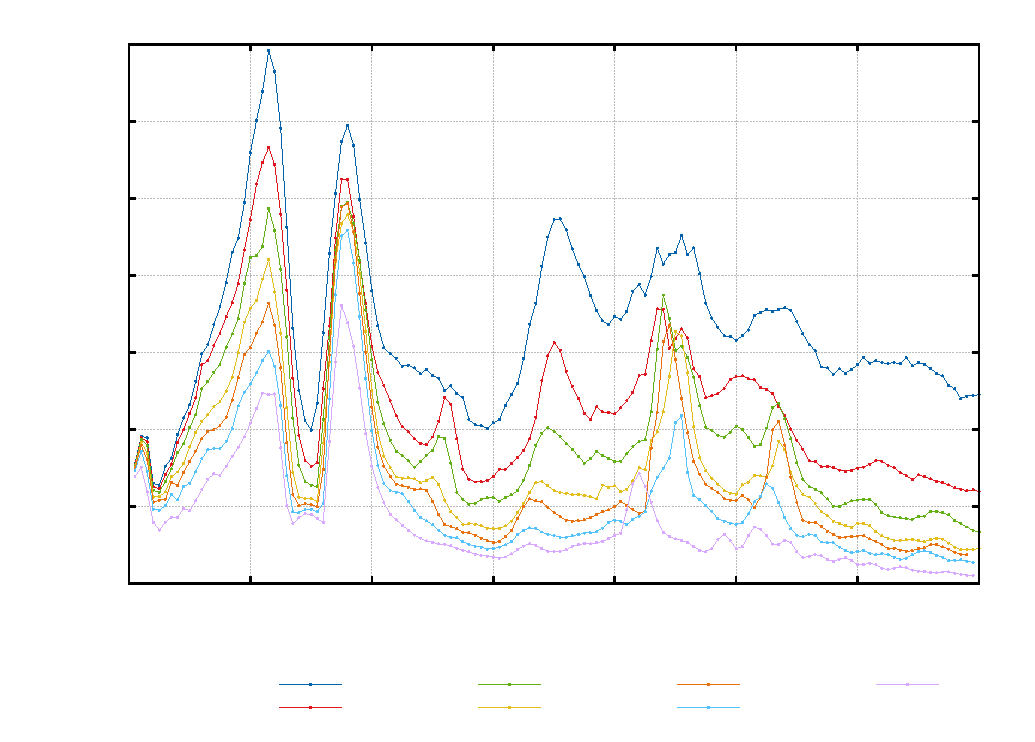
\includegraphics{et_vis}}%
    \gplfronttext
  \end{picture}%
\endgroup

\caption{Wykres energii kinetycznej cząstek od czasu $E_c(t)$ w zależności od współczynnika lepkości $\mu$}
\label{fig:plot_viscosity}
\end{figure}

\par
Na wykresie \eqref{fig:plot_viscosity} widać jak energia cząsteczek jest tłumiona przez siłę lepkości. Lepkość wpływa również na przebieg symulacji co widać na wykresie jako różnice w przebiegu krzywych i różne miejsca występowania ekstremów lokalnych.
\par

\begin{figure}[H]
% GNUPLOT: LaTeX picture with Postscript
\begingroup
  \makeatletter
  \providecommand\color[2][]{%
    \GenericError{(gnuplot) \space\space\space\@spaces}{%
      Package color not loaded in conjunction with
      terminal option `colourtext'%
    }{See the gnuplot documentation for explanation.%
    }{Either use 'blacktext' in gnuplot or load the package
      color.sty in LaTeX.}%
    \renewcommand\color[2][]{}%
  }%
  \providecommand\includegraphics[2][]{%
    \GenericError{(gnuplot) \space\space\space\@spaces}{%
      Package graphicx or graphics not loaded%
    }{See the gnuplot documentation for explanation.%
    }{The gnuplot epslatex terminal needs graphicx.sty or graphics.sty.}%
    \renewcommand\includegraphics[2][]{}%
  }%
  \providecommand\rotatebox[2]{#2}%
  \@ifundefined{ifGPcolor}{%
    \newif\ifGPcolor
    \GPcolortrue
  }{}%
  \@ifundefined{ifGPblacktext}{%
    \newif\ifGPblacktext
    \GPblacktextfalse
  }{}%
  % define a \g@addto@macro without @ in the name:
  \let\gplgaddtomacro\g@addto@macro
  % define empty templates for all commands taking text:
  \gdef\gplbacktext{}%
  \gdef\gplfronttext{}%
  \makeatother
  \ifGPblacktext
    % no textcolor at all
    \def\colorrgb#1{}%
    \def\colorgray#1{}%
  \else
    % gray or color?
    \ifGPcolor
      \def\colorrgb#1{\color[rgb]{#1}}%
      \def\colorgray#1{\color[gray]{#1}}%
      \expandafter\def\csname LTw\endcsname{\color{white}}%
      \expandafter\def\csname LTb\endcsname{\color{black}}%
      \expandafter\def\csname LTa\endcsname{\color{black}}%
      \expandafter\def\csname LT0\endcsname{\color[rgb]{1,0,0}}%
      \expandafter\def\csname LT1\endcsname{\color[rgb]{0,1,0}}%
      \expandafter\def\csname LT2\endcsname{\color[rgb]{0,0,1}}%
      \expandafter\def\csname LT3\endcsname{\color[rgb]{1,0,1}}%
      \expandafter\def\csname LT4\endcsname{\color[rgb]{0,1,1}}%
      \expandafter\def\csname LT5\endcsname{\color[rgb]{1,1,0}}%
      \expandafter\def\csname LT6\endcsname{\color[rgb]{0,0,0}}%
      \expandafter\def\csname LT7\endcsname{\color[rgb]{1,0.3,0}}%
      \expandafter\def\csname LT8\endcsname{\color[rgb]{0.5,0.5,0.5}}%
    \else
      % gray
      \def\colorrgb#1{\color{black}}%
      \def\colorgray#1{\color[gray]{#1}}%
      \expandafter\def\csname LTw\endcsname{\color{white}}%
      \expandafter\def\csname LTb\endcsname{\color{black}}%
      \expandafter\def\csname LTa\endcsname{\color{black}}%
      \expandafter\def\csname LT0\endcsname{\color{black}}%
      \expandafter\def\csname LT1\endcsname{\color{black}}%
      \expandafter\def\csname LT2\endcsname{\color{black}}%
      \expandafter\def\csname LT3\endcsname{\color{black}}%
      \expandafter\def\csname LT4\endcsname{\color{black}}%
      \expandafter\def\csname LT5\endcsname{\color{black}}%
      \expandafter\def\csname LT6\endcsname{\color{black}}%
      \expandafter\def\csname LT7\endcsname{\color{black}}%
      \expandafter\def\csname LT8\endcsname{\color{black}}%
    \fi
  \fi
  \setlength{\unitlength}{0.0500bp}%
  \begin{picture}(9636.00,7370.00)%
    \gplgaddtomacro\gplbacktext{%
      \csname LTb\endcsname%
      \put(946,1144){\makebox(0,0)[r]{\strut{} 0}}%
      \csname LTb\endcsname%
      \put(946,2336){\makebox(0,0)[r]{\strut{} 20}}%
      \csname LTb\endcsname%
      \put(946,3528){\makebox(0,0)[r]{\strut{} 40}}%
      \csname LTb\endcsname%
      \put(946,4721){\makebox(0,0)[r]{\strut{} 60}}%
      \csname LTb\endcsname%
      \put(946,5913){\makebox(0,0)[r]{\strut{} 80}}%
      \csname LTb\endcsname%
      \put(946,7105){\makebox(0,0)[r]{\strut{} 100}}%
      \csname LTb\endcsname%
      \put(1078,924){\makebox(0,0){\strut{} 0}}%
      \csname LTb\endcsname%
      \put(2244,924){\makebox(0,0){\strut{} 0.4}}%
      \csname LTb\endcsname%
      \put(3410,924){\makebox(0,0){\strut{} 0.8}}%
      \csname LTb\endcsname%
      \put(4576,924){\makebox(0,0){\strut{} 1.2}}%
      \csname LTb\endcsname%
      \put(5741,924){\makebox(0,0){\strut{} 1.6}}%
      \csname LTb\endcsname%
      \put(6907,924){\makebox(0,0){\strut{} 2}}%
      \csname LTb\endcsname%
      \put(8073,924){\makebox(0,0){\strut{} 2.4}}%
      \csname LTb\endcsname%
      \put(9239,924){\makebox(0,0){\strut{} 2.8}}%
      \csname LTb\endcsname%
      \put(176,4124){\rotatebox{-270}{\makebox(0,0){\strut{}$E_c(t)$}}}%
      \put(5158,594){\makebox(0,0){\strut{}$t$}}%
    }%
    \gplgaddtomacro\gplfronttext{%
      \csname LTb\endcsname%
      \put(2524,173){\makebox(0,0)[r]{\strut{}$\mu = 0.5$}}%
      \csname LTb\endcsname%
      \put(4303,173){\makebox(0,0)[r]{\strut{}$\mu = 1.5$}}%
      \csname LTb\endcsname%
      \put(6082,173){\makebox(0,0)[r]{\strut{}$\mu = 2.5$}}%
      \csname LTb\endcsname%
      \put(7861,173){\makebox(0,0)[r]{\strut{}$\mu = 5.0$}}%
    }%
    \gplbacktext
    \put(0,0){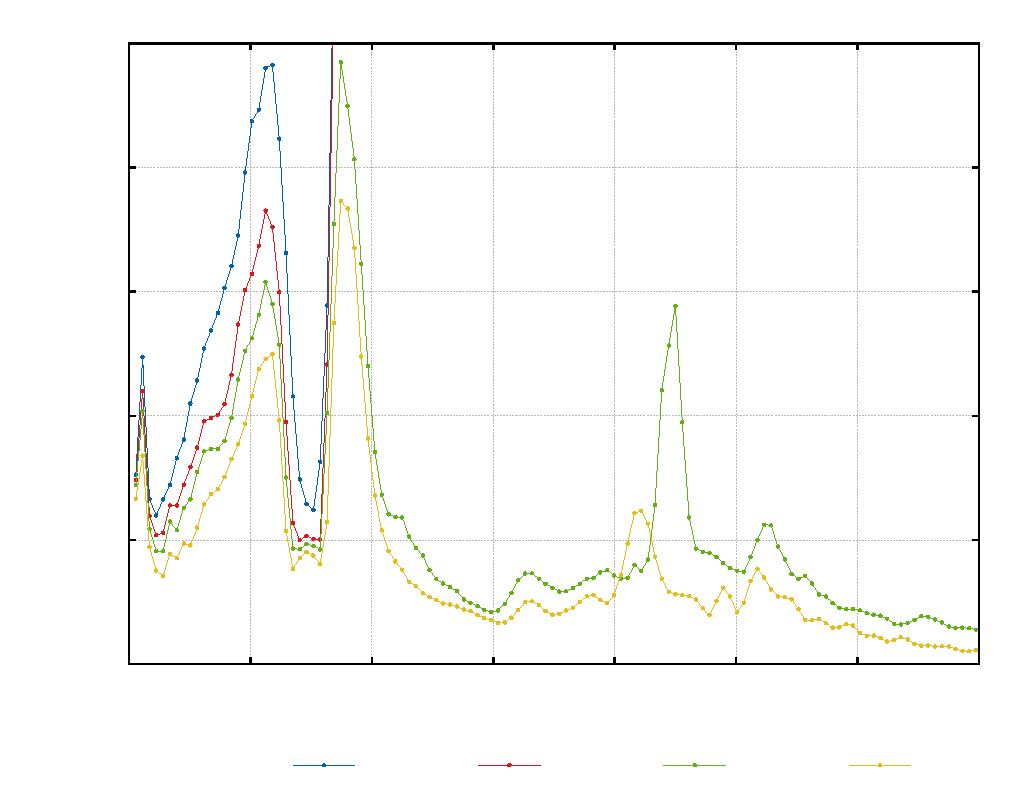
\includegraphics{et_vis_hdt}}%
    \gplfronttext
  \end{picture}%
\endgroup

\caption{Wykres energii kinetycznej cząstek od czasu $E_c(t)$ w zależności od współczynnika lepkości $\mu$, przy dużym kroku czasowym $\Delta t$ = 0.005}
\label{fig:plot_viscosity_highdt}
\end{figure}

\par
Wykres \eqref{fig:plot_viscosity_highdt} obrazuje efekt `wygładzający' siły lepkości. Siła ta przyciąga poszczególne cząsteczki do siebie przez co ich zdolności do nabierania prędkości są ograniczone. Ten efekt pozwala na przeprowadzenie stabilnej symulacji dla większego kroku czasowego. Jednak, jak można zauważyć na wykresie, przy średnich wartościach stałej siły lepkości $\mu$ ($0.5$ i $1.5$) i sporym kroku czasowym wybuch symulacji jest nieuchronny (następuje przy $t$ wynoszącym ok. $0.65$).

\subsubsection{Napięcie powierzchniowe}

\paragraph{}
W równaniu \eqref{eqn:sph_force_surface_tension} występuje stała $\sigma$ modulująca siłę przyciągania do siebie cząstek znajdujących się na powierzchni płynu. Jej większa wartość powoduje zwiększenie się tej siły.
Wartość progu $l$ funkcjonującego w równaniu \eqref{eqn:sph_force_surface_tension_threshold} ma jedynie ustrzec przed dzieleniem przez bardzo małe wartości co negatywnie wpływa na stabilność symulacji. Wartość progu powinna być niska aby zachować naturalność działania siły napięcia powierzchniowego.
\par